\documentclass[10pt]{article}
\usepackage[utf8]{inputenc}
\usepackage[activeacute,spanish]{babel}
\usepackage[left=1.5cm,top=1.5cm,right=1.5cm, bottom=1.5cm,letterpaper, includeheadfoot]{geometry}

\usepackage{amssymb, amsmath, amsthm}
\usepackage{graphicx}
\usepackage{hyperref}
\usepackage{lmodern,url}
\usepackage{paralist} %util para listas compactas
\usepackage{xcolor}
\usepackage{bbm}
\usepackage{mathrsfs}
\usepackage{bbm}

%========PAQUETES AGREGADOS===========
%Pseudocodigo
\usepackage{pseudocode}
\usepackage[portuguese, boxruled]{algorithm2e}
\usepackage{wrapfig}
\usepackage{multicol}
\usepackage{graphicx}
\usepackage{caption}
\usepackage{subcaption}
%\captionsetup[table]{labelformat=empty}
\captionsetup[subfigure]{labelformat=empty}
\usepackage{cancel}
\usepackage{tikz}
\def\checkmark{\tikz\fill[scale=0.4](0,.35) -- (.25,0) -- (1,.7) -- (.25,.15) -- cycle;} 
%====================================

\usepackage{fancyhdr}
\pagestyle{fancy}
\fancypagestyle{plain}{%
\fancyhf{}
\lhead{\footnotesize\itshape\bfseries\rightmark}
\rhead{\footnotesize\itshape\bfseries\leftmark}
}


% macros
\newcommand{\Q}{\mathbb Q}
\newcommand{\R}{\mathbb R}
\newcommand{\N}{\mathbb N}
\newcommand{\Z}{\mathbb Z}
\newcommand{\C}{\mathbb C}
\newcommand{\BigO}{\mathcal{O}}
%Teoremas, Lemas, etc.
\theoremstyle{plain}
\newtheorem{teo}{Teorema}
\newtheorem{lem}{Lema}
\newtheorem{prop}{Proposición}
\newtheorem{cor}{Corolario}
\newtheorem{obs}{Observación}
\newtheorem{ej}{Ejemplo}
\renewcommand{\qedsymbol}{\rule{0.7em}{0.7em}}
\renewenvironment{proof}{{\bfseries \noindent Demostración}}{ \qed \\}


\theoremstyle{definition}
\newtheorem{defi}{Definición}
% fin macros


\newcommand{\catnum}{11} %numero de catedra
\newcommand{\fecha}{13 de Septiembre 2016 }

%%%%%%%%%%%%%%%%%%

%Macros para este documento
\newcommand{\cin}{\operatorname{cint}}



\begin{document}
%Encabezado
\fancyhead[L]{Facultad de Ciencias Físicas y Matemáticas}
\fancyhead[R]{Universidad de Chile}
\vspace*{-1.2 cm}
\begin{minipage}{0.6\textwidth}
\begin{flushleft}
\hspace*{-0.5cm}\textbf{MA3402-1 Estadística. Primavera 2016}\\
\hspace*{-0.5cm}\textbf{Profesor:} Raul Gouet\\
\hspace*{-0.5cm}\textbf{Escriba:} Manuel Cáceres\\
\hspace*{-0.5cm}\textbf{Fecha:} \fecha
\end{flushleft}
\end{minipage}
\begin{minipage}{0.36\textwidth}
\begin{flushright}

\includegraphics[scale=0.3]{imagenes/fcfm_dcc}
\end{flushright}
\end{minipage}
\bigskip
%Fin encabezado

\begin{center}
\LARGE\textbf{Clase \catnum}
\end{center}
\section{Hipótesis Compuestas}
Recordemos quel TNP es el óptimo para el problema del tipo $H_{0}: \theta = \theta_{0}$ vs $H_{1}: \theta = \theta_{1}$ con $\Theta = \{\theta_{0}, \theta_{1}\}$ en el sentido de tener la mejor potencia posible en la clase $\tau_{\alpha}$ (de nivel $\alpha$).\\
	
\textbf{¿Cómo abordar los problemas más realistas (cercanos a la aplicaciones) donde $H_{0}$ o $H_{1}$ o ambos son compuestas?}\\

Veremos que el TNP puede servir (sirve) en problemas compuestos unilaterales.\\
Recordemos que el TNP $\phi^*$ para $H_{0}: \mu = \mu_{0}$ vs $H_{1}: \mu = \mu_{1}, \mu_{1}>\mu_{0}$ en el modelo gaussiano, basados en la misma muestra iid $X_{1},\ldots,X_{n}$.\\
Sabemos que $\phi^*(X)=1 \Leftrightarrow \bar{X} \ge \mu_{0} + \frac{\sigma}{\sqrt{n}}\phi^{-1}(1-\alpha)$.\\
Sabemos que $\phi^* \in \tau_{\alpha} (\alpha_{\phi^*}(\mu_{0}) = \alpha)$ y que:
\begin{align*}
\alpha_{\phi^*}(\mu_{1}) = \underbrace{(1-\phi)}_{funcion} \left(\frac{\sqrt{n}(\mu_{0}-\mu_{1})}{\sigma}+ \phi^{-1}(1-\alpha)\right)
\end{align*}
con $\sigma_{\phi^*}(\mu_{1}) \ge \alpha_{\phi}(\mu_{1}), \forall \phi \in \tau_{\alpha}$.\\

Pensemos en el problema unilateral (una cola) $P'$, $H_{0}: \underbrace{\mu = \mu_{0}}_{simple}$ vs $H_{1}: \underbrace{\mu > \mu_{0}}_{compuesta}$, se entiende que $\Theta = [\mu_{0},\infty[$.\\
Veamos que pasa si usamos el TNP $\phi^*$ en este problema. Primero notemos que $\phi^* \in \tau_{\alpha}$ (los tests de nivel $\alpha$ para $P'$).\\
\begin{align*}
 \phi \in \tau_{\alpha} & \Leftrightarrow \mathbb{P}_{\mu}(x\in \mathbb{R}_{\phi}) \le \alpha \forall \mu \in \Theta_{0} = \{\mu_{0}\}\\
 & \Leftrightarrow \mathbb{P}_{\mu_{0}}(x\in \mathbb{R}_{\phi}) \le \alpha
\end{align*}
Por definición de TNP sabemos que $\alpha_{\phi^*}(\mu) \ge \alpha_{\phi}(\mu), \forall \mu \ge \mu_{0}, \forall \phi \in \tau_{\alpha}$, de donde se ve que $\phi^*$ es test UMP de nivel $\alpha$ para el problema $P'$. SALIÓ GRATIS!\\

Se ha resuelto el problema de encontrar test UMP para $P'$ $H_{0}: \mu=\mu_{0}$ vs $H_{1}: \mu>\mu_{0}$.\\
Pasemos al problema $P''$ $H_{0}: \mu \le \mu_{0}$ vs $H_{1}: \mu>\mu_{0}$ y veamos si $\phi^*$ sigue valiendo en este caso.\\
La clase $\tau_{\alpha}$ tiene los $\phi$ tales que:
\begin{align*}
\sup_{\mu\le\mu_{0}}\mathbb{P}_{\mu}(\phi(X)=1) \le \alpha & \land \phi^* \in \tau_{\alpha}\\
\sup_{\mu\le \mu_{0}} \mathbb{E}_{\mu}(\phi^*(X)) &= \sup_{\mu\le \mu_{0}} \underbrace{\mathbb{P}_{\mu}(\bar{X}\ge \frac{\sigma}{\sqrt{n}}\phi^{-1}(1-\alpha) + \mu_{0})}_{\alpha_{\phi^*}(\mu) = (1-\phi)\left(\frac{\sqrt{n}}{\sigma}(\mu_{0}-\mu )+ \phi^{-1}(1-\alpha)\right)} 
\end{align*}
$\alpha_{\phi^*}(\mu)$ es función creciente y continua de $\mu$ por lo que alcanza el supremo en $\mu_{0}$.\\
$\mathbb{P}_{\mu_{0}}(\ldots) \le \alpha$ es cierto, pues $\mathbb{P}(\phi^*(X)=1)=1$ así fue deducido.\\
Como en el rango $(\mu_{0},\infty)$ el gana a $\phi^*$,entonces resulta que es UMP de nivel $\alpha$ de nivel $P''$.\\

Existen muchos problemas unilaterales (con parametro $\mathbb{R}$) donde el TNP puede ser usado y constituye un test UMP.\\

Por suspuesto podemos explorar problemas unilaterales del lado izquierdo, por ejemplo: $H_{0}: \mu = \mu_{0}$ versus $H_{1}: \mu<\mu_{1}$ o $H_{0}: \mu \ge \mu_{0}$ versus $H_{1}: \mu=\mu_{1}$.\\

En el caso $H_{0}: \mu=\mu_{0}$ versus $H_{1}: \mu=\mu_{1} (\mu_{1}<\mu_{0})$ tiene un TNP $\phi_{i}^*(X)=1 \Leftrightarrow \bar{X}\le k_{\alpha}$(el subíndice i indica por la izquierda).\\

Se muestra que $\phi^*_{i}$ es UMP en todos estos casos unilaterales.\\

Que pasa en el siguiente problema ``bilateral'': $H_{0}: \underbrace{\mu=\mu_{0}}_{simple}$ versus $H_{1}: \underbrace{\mu\not = \mu_{0}}_{compuesta}, \Theta = \mathbb{R}, \Theta_{0}=\{\mu_{0}\}$ .\\

En este problema el TNP $\phi^*_{i}$ y $\phi^*_{d}$ fracasan estrepitosamente.\\
Si usamos $\phi_{d}^*$, entonces rechazamos $H_{0}:\mu=\mu_{0}$ si $\bar{X}\ge \frac{\sigma}{\sqrt{n}}\phi^{-1}(1-\alpha) + \mu_{0}$ lo cual estaría bien en el rango $(\mu_{0},\infty)$ de $H_{1}$.\\

¿Qué pasa con $\phi^*_{d}$ en $(-\infty, \mu_{0})$? Bueno, ocurre que la potencia $\alpha_{\phi^*_{d}}(\mu) \le \alpha$, lo cual es absurdo.\\

¿Sería $\phi^*_{d}$ UMP para $H_{0}: \mu=\mu_{0}$ versus $H_{1}: \mu \not = \mu_{0}$? La respuesta es no pues el otro TNP $\phi^*_{i}$ el gana a $\phi^*_{d}$ en $(-\infty, \mu_{0})$.\\

Sabiendo que el TNP es único (esencialmente) entonces concluímos que no existe test UMP de nivel $\alpha$ para $H_{0}: \mu = \mu_{0}$ versus $H_{1}: \mu \not = \mu_{0}$.\\

¿Qué hacemos entonces?\\
Es razonable pensar que rechazamos $H_{0}: \mu = \mu_{0}$ en beneficio de $H_{1}: \mu \not = \mu_{0}$ cuando $|\bar{X}-\mu_{0}|$ sea grande. Definimos el test $\phi$ tal que $\phi(X)=1 \Leftrightarrow |\bar{X}-\mu_{0}|\ge k_{\alpha}$ y lo hacemos de nivel $\alpha$, esto no es un UMP (no existe). Calculamos $k_{\alpha}$ resolviendo:
\begin{align*}
&\mathbb{P}_{\mu_{0}}\left(|\bar{X}-\mu_{0}|>k_{\alpha}\right) = \alpha\\
 \Leftrightarrow & \mathbb{P}_{\mu_{0}}\left(\frac{|\bar{X}-\mu_{0}|}{\sigma/\sqrt{n}}\ge k_{\alpha}\frac{\sqrt{n}}{\sigma}\right) = \alpha
\end{align*}
\begin{center}
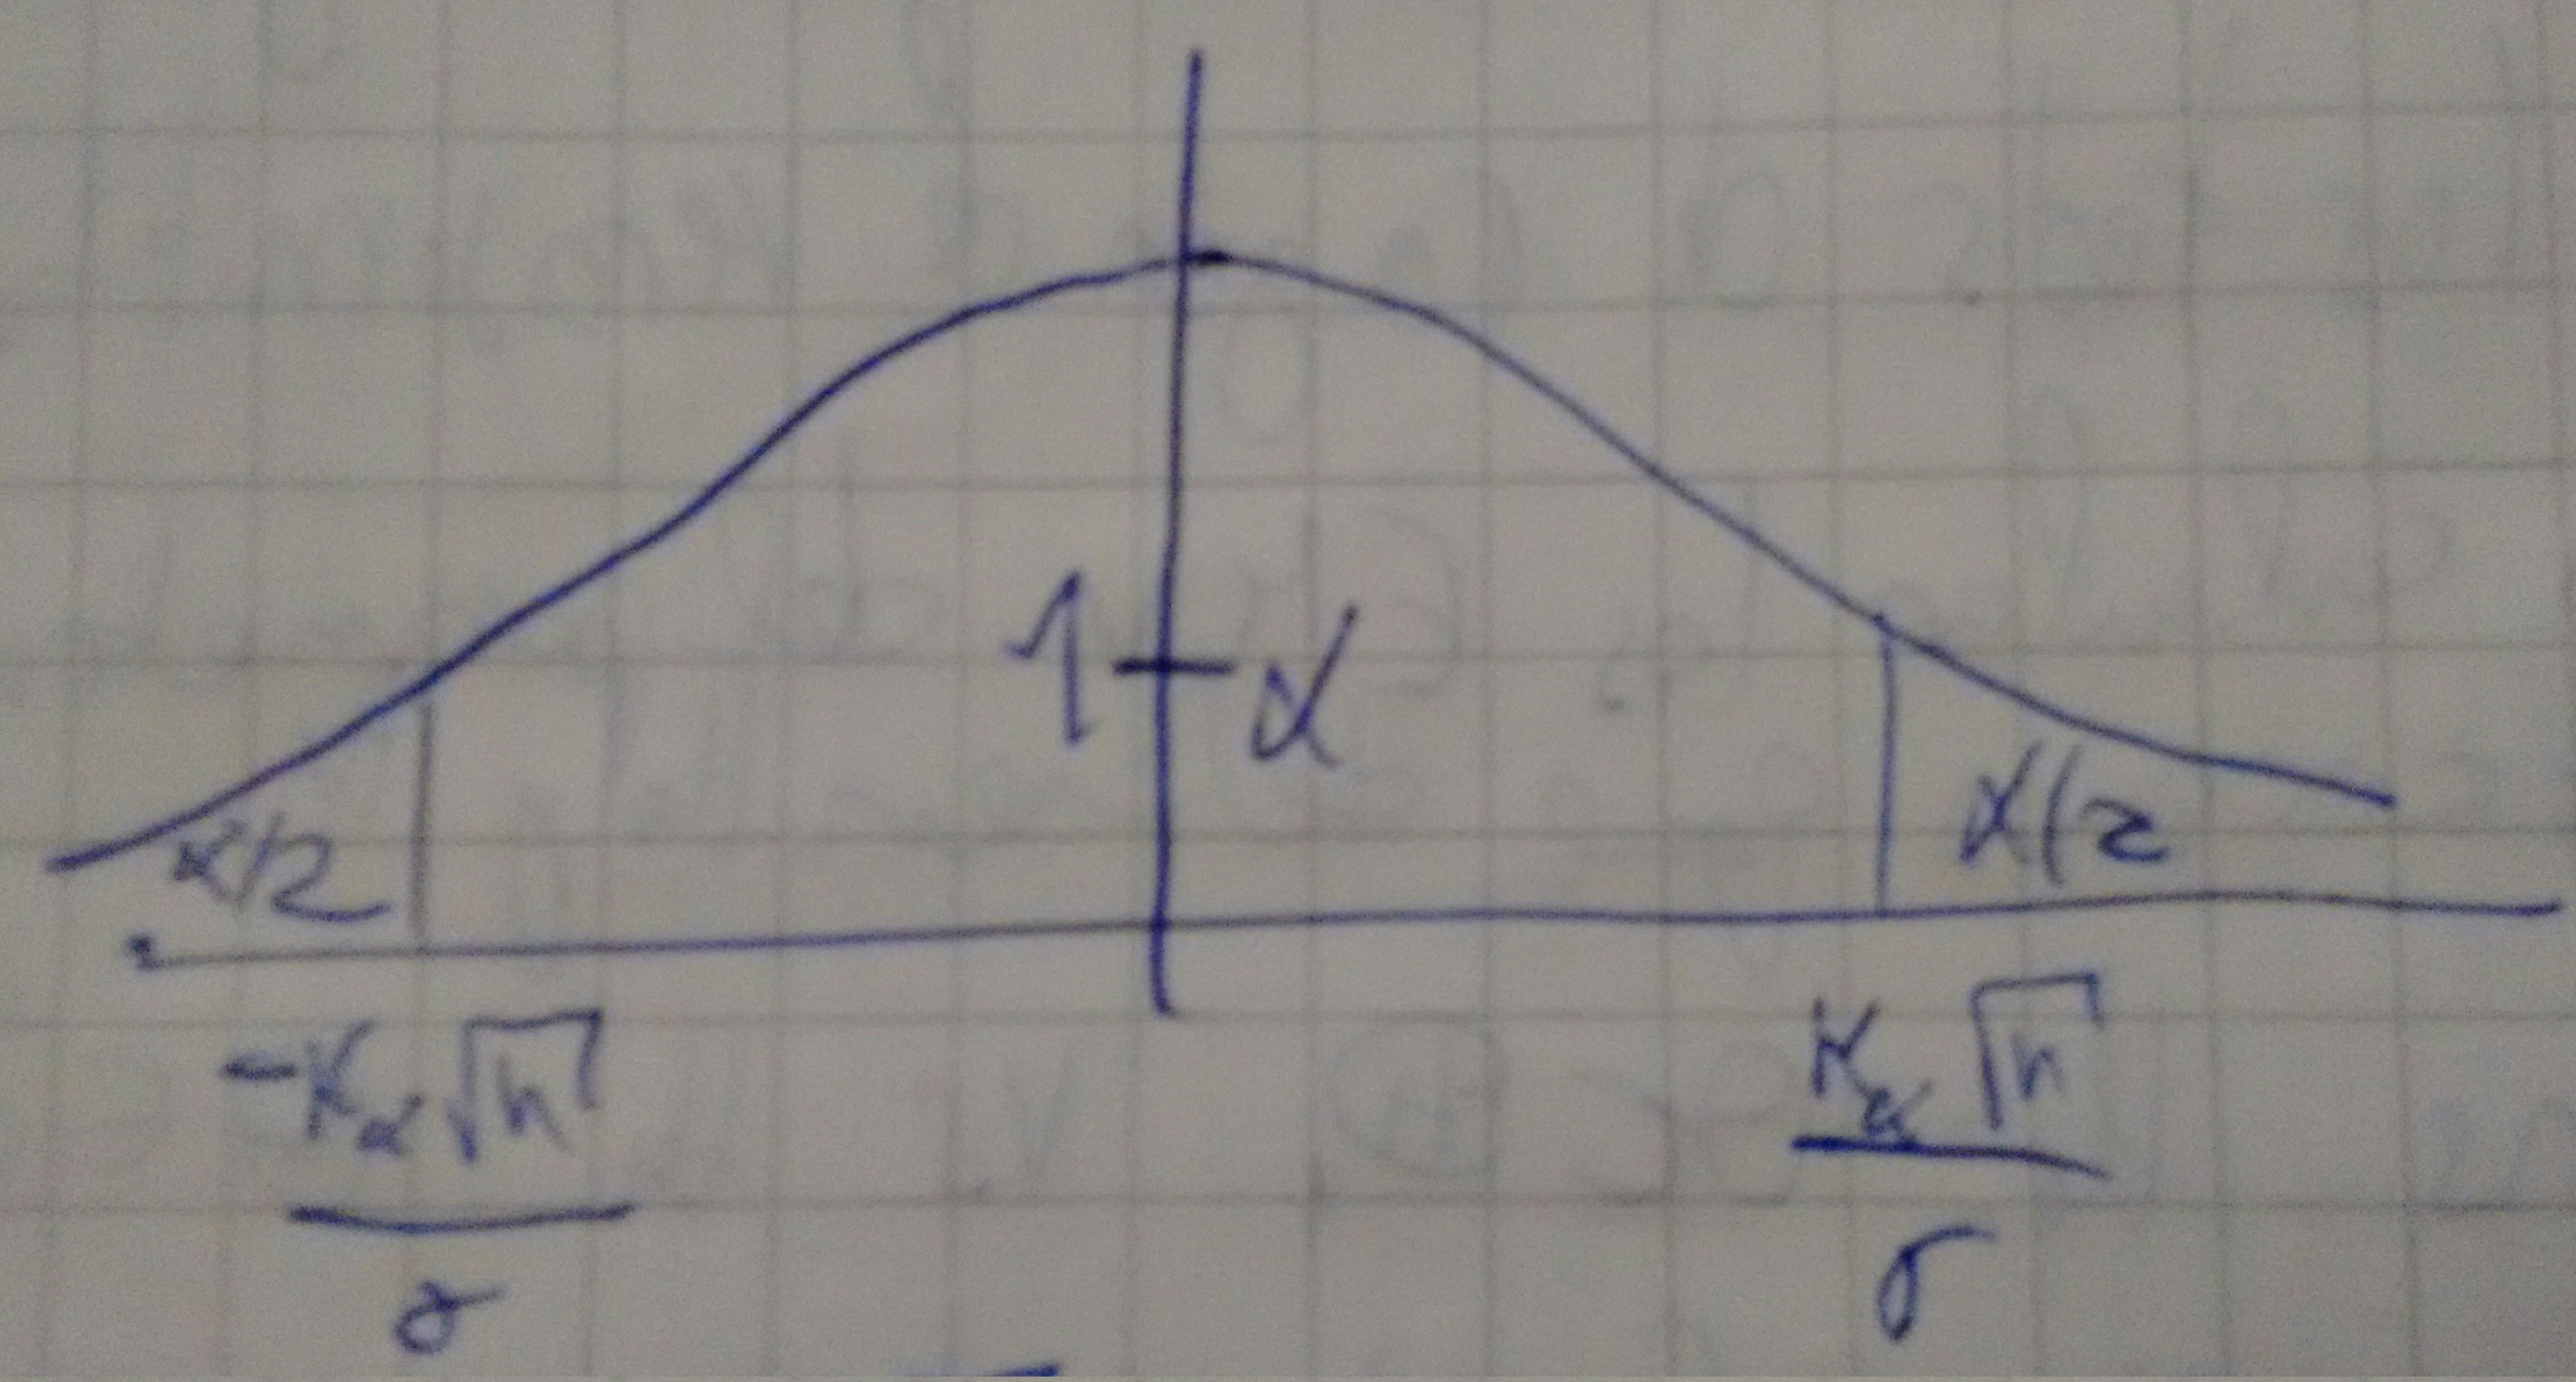
\includegraphics[scale=0.1]{imagenes/bilateral.jpg}
\end{center}
\begin{align*}
\Rightarrow & \frac{k_{\alpha}\sqrt{n}}{\sigma} = \phi^{-1}(1-\alpha/2)
\end{align*}
Luego, $\phi$ rechaza si $|\bar{X}-\mu_{0}| \ge \frac{\sigma}{\sqrt{n}}\phi^{-1}(1-\alpha/2) \Leftrightarrow \mu_{0} \not \in [\bar{X}-\frac{\sigma}{\sqrt{n}}\phi^{-1}(1-\alpha/2), \bar{X}+\frac{\sigma}{\sqrt{n}}\phi^{-1}(1-\alpha/2)]$.\\

Este test razonable de nivel $\alpha$ no es UMP, pero se puede demostrar que si es UMP en la subclase de los tests insesgados de nivel $\alpha$.
\section{Test insesgado}
Un test cuya probabilidad de rechazar bajo $H_{1}$ es mayor o igual que la probabilidad de rechazar bajo $H_{0}$ se llama insesgado.\\
Si $\phi$ es de nivel $\alpha$ para $H_{0}: \theta \in \Theta_{0}$ versus $H_{1}: \theta \in \Theta_{1}$ resulta que $\alpha_{\phi}(\theta) \ge \alpha, \forall \theta \in \Theta_{0}$. Su $\phi$ es insesgado entonces $\alpha_{\phi}(\theta) \ge \alpha, \forall \theta \in \Theta_{1}$.\\

Vamos hacia un método general para diseñar tests cuyas cualidades no están garantizadas. Se trata de los tets de razón de verosimilitud.\\
La idea es calcular los EMV del parámetro $\theta$ sujeto a las restricciones que definen $H_{0}\ y\ H_{1}$.\\
Consideramos $H_{0}: \theta \in \Theta_{0}$ versus $H_{1}: \theta \in \Theta_{1}$ y definimos:
\begin{align*}
\lambda(X) = \frac{\sup_{\theta \in \Theta_{1}} f_{\theta}(X)}{\sup_{\theta \in \Theta_{0}} f_{\theta}(X)}
\end{align*}
Sea $\mathbb{R}=\{x\in\mathfrak{X}; \lambda(X) \ge k_{\alpha}\}$, donde $k_{\alpha}$ se calcula de manera que
\begin{align*}
\sup_{\theta \in \Theta_{0}} \mathbb{P}_{\theta}\left(\lambda(X) \ge k_{\alpha}\right) \le \alpha
\end{align*}
y $\phi$ se define como $\phi(X) = 1 \Leftrightarrow x \in \mathbb{R}$.\\

Es TNP coincide con el test de razón de verosimilitud (TRV) con la salvedad de igualar a $\alpha$ la probabilidad de error tipo I.\\

El primer ejemplo que estudiaremos es:
\begin{itemize}
\item $H_{0}: \mu = \mu_{0}$ versus $H_{1}: \mu > \mu_{0}$ (que ya sabemos resolver y existe UMP)
\item $H_{0}: \mu = \mu_{0}$ versus $H_{1}: \mu \not =\mu_{0}$
\end{itemize}
\end{document}